
%*****************************************************************************************
%*********************************** First Chapter ***************************************
%*****************************************************************************************

\chapter{Introduction}  %Title of the First Chapter

\ifpdf
    \graphicspath{{Chapter1/Figs/Raster/}{Chapter1/Figs/PDF/}{Chapter1/Figs/}}
\else
    \graphicspath{{Chapter1/Figs/Vector/}{Chapter1/Figs/}}
\fi


A systems level understanding of biology has always been in the back
of the minds of biologists since it is this distributed information
processing that ultimately gives rise to phenotype and macroscopic
behaviour to sustain life. Perhaps the apparent great complexity at
which these systems operate or the lack of relevant experimental data
has made Biology as a discipline to focus its efforts on the
understanding of the information processing capabilities and inner
workings of the individual constituent components of these
systems. Relatively recent technological advances however have led to
an accumulation of a wealth of data sheding light into the interactions
between components, their dependencies and the constraints these
impose. While understanding the individual components, genes,
proteins, is still important these new data sources have led to a shift
of focus to the study of biological systems in their entirety. In
doing so we realised that the most important aspect of these systems
is not the inner workings of the individual components but rather the
interactions between them.

Traditionally biology has not used any formal methods to explain
things and perhaps that was not needed when we were dealing with
single entities. As the systems grew in size it became apparent that
some change in direction was needed to handle the increased complexity
and get a coherent story. Systems Biology tries to fill this gap by
bringing in practises from other more traditionally formal fields like
Mathematics, Physics, Computer Science(\citet{kitano2002systems, ideker2001new}).

Early attempts to capture the more complex picture painted by the
increase in the number of components were to use static diagrams to
capture the interactions and dependencies between them. These diagrams
have been widely used in Biochemistry and particularly in metabolism
since the species conversion process that takes place in metabolic
pathways can easily be seen as a path or paths through these diagrams going from
one metabolite to the next(see for example
Figure~\ref{fig:fa_synthesis_pathway}). Now these diagrams are very important and
they contain important knowledge about our understanding of the
operations of biological systems. There exist databases that contain our current
understanding of a particular system annotated with information from
different sources and these are particularly popular for metabolic
pathways (see \citet{kanehisa2000kegg},
\citet{pharkya2003review}). These static diagrams are an example of
bottoms-up approach in System Biology which is a data-driven process,
starting from some large experimental datasets we extract biological
information. This is in contrast to the top-down approach where
starting from detailed knowledge about a system we try to build a
mechanistic explanation of it(\citet{schneider2013understanding}). 

\begin{figure}[htbp!] 
\centering    
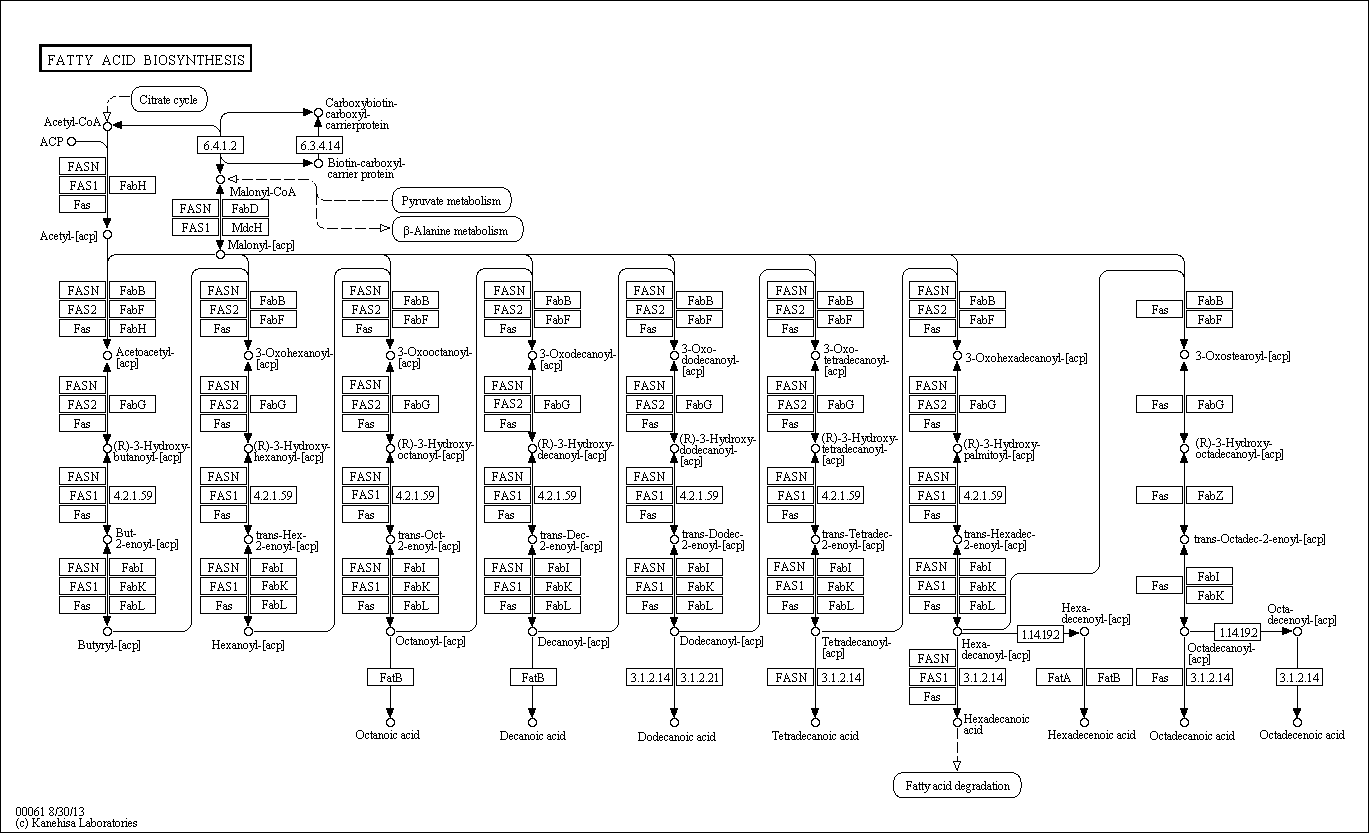
\includegraphics[width=1.0\textwidth]{fa_synthesis_pathway}
\caption[Fatty Acid synthesis pathway]{Fatty acid synthesis pathway
  captured by the standard diagrammatic language used to capture
  interactions between components in a biological system. This was
  taken from KEGG a database which contains current knowledge about
  the working of these systems(from experiments for example)
  integrated with data from multiple sources.}
\label{fig:fa_synthesis_pathway}
\end{figure}

Despite the importance of the bottom-up static diagrams they paint a
very static picture of the system which is not enough to gain a full
understanding of the system. What is often needed is a dynamic picture
of the system with a top-down mechanistic model to observe things that
are not possible from a static
picture like control mechanisms, dynamic interactions between
components over time, and dynamic responses to external stimuli.


\section{Dynamical systems theory and Flux Balance Analysis}
This need to look into dynamic behaviour led to Dynamical System
theory which based on its success in Physics has found its way in many
other fields. Dynamical system theory captures the relationship
between continuous quantities in difference-differential equations
which describe the evolution of state variables in terms of changes
in other state variables and even themselves thus capturing the
interaction element. Since the time of Newton and classical mechanics
,where these ideas originated, the toolbox of dynamical systems theory
has grown to include techniques for qualitative understanding of
system without the need to solve them either numerically or
analytically. 

In biochemistry each species in the system is represented by its 
concentration leading to a differential equation for each species. The
rate of change of the concentration of a species is described in terms
of in flows- increasing the rate of change(production)- and out flows
- decreasing the rate of change(degradation). These flows can be
dependent on the concentrations of other variables(species) which
participate in the same biochemical reactions. Consider for example a
system with $n$ components which we can group into the global state of
the system $\mathbf{x} = (x_1, x_2, \dots x_n)$. All the reactions
that take place in the system change, in discrete levels, the numbers
of molecules of the species:

\begin{align*}
\mathbf{x} &\overset{r_1(\mathbf{x})}{\longrightarrow} \mathbf{x} +
\mathbf{\delta_1}\\
\mathbf{x} &\overset{r_2(\mathbf{x})}{\longrightarrow} \mathbf{x} +
\mathbf{\delta_2}\\
\vdots \\
\mathbf{x} &\overset{r_m(\mathbf{x})}{\longrightarrow} \mathbf{x} +
\mathbf{\delta_m}
\end{align*}
So for every reaction we have one such rule and $\delta_k$ are the
discrete levels by which the species change for every reaction. Each
reaction has an associated and possible state dependent rate $r_k(x)$
which is the expected number of times it takes place in a time
unit. The in-flows are the positive deltas and out-flows the negative
ones. The differential equation describing the evolution of the average numbers
of  species $i$ is then the sum of the in
and out flows over all reactions in the system:

\begin{equation*}
\frac{dx_i}{dt} = \sum_{m} r_m(\mathbf{x})\delta_{mi}
\end{equation*}

Usually this formulation of the problem leads to integration with a
numerical ODE solver of the above system to get the dynamic behaviour
of the system. The usual problem mathematical biologists face is that
the reaction rate function(the $r_k(\mathbf{x})$s) contain parameter
constants that are not usually known. 
%Maybe write another problem here

In the contex of metabolic systems however there is a mathematical technique however, called Flux Balance
Analysis, that is used to compute these flows without explicit
knowledge of these parameters by making some assumptions about the
system to simplify the problem. If we assume that that metabolites
cannot accumulate within the cell and their levels are more or less
balanced then the system is at steady-state. The steady-state assumption means that the average positive flux-defined as the sum of
all the in-flows- and the average negative flux-defined as the sum of
all the out-flows- that means that all the for every species its rate
of change, which is the sum of all flows(negative and
positive), is equal to 0. Solving for the fluxes leads to a linear equation for each
species. For a more concise notation all the $\delta_{nm}$ are
packaged into a matrix $\mathbf{S}$, traditionally called the Stoichiometric
matrix and the fluxes in a vector $\mathbf{r}$. Then the problem
becomes solving the system $\mathbf{Sr} = \mathbf{0}$ to calculate the
fluxes $\mathbf{r}$ through our system of interest. The only problem
with this formulation of the problem is that the system is
underdetermined since usually the number of reactions is higher than
the number of species. To solve this the solution space is constrained
with the use of an objective function which leads to a linear
programming problem formulation which is easily solvable.

Flux balance analysis is a very powerful technique since it allows us
to overcome the problem of the rate parameters and calculate the
fluxes through the system in a computationally efficient way. It is
not without its limitations though.

%Say stuff about the limitations
\section{Challenge of lipid metabolism}
%I need to motivate stochastic simulations better here and also write
%a bit more(with references) about why lipid metabolism is important

Lipid metabolism is particularly important topic since it is linked
with several disorders and diseases. The fact that it is has
complicated regulatory mechanisms has made getting a systems level
understaning of it very important. In fact many system biology
attempts have been made to get even a genome-wide picture of metabolism in
mammals or other organisms. We think that lipid metabolism Systems
Biology modelling might benefit from a different type of approach than
the deterministic picture offered by dynamic systems theory and
consequently FBA. The iterative nature of many of its subsystems, like
the Fatty Acid Synthesis/Elongation system which we examine in this
study, along with the need to understand more local regulatory
mechanims calls for a reaction-centric view of the system.

A biochemical system, like the one given in the previous section,
consisting of a number of reactions that alter the integer numbers of
molecules of the species describes a random process and a Continuous
Time Markov Chain in particular. The differential equations we used as
a basis for FBA are a just
deterministic view of the average behaviour. The dynamics of the
system can be set in motion inside a computer using the Gillespie
exact simulation algorithm which creates sample
time-series. Statistical information like the strenth of the
fluctuations (normalised variance) can be computed by collecting a lot
of these traces.

In this study we use an alternative more formal language with an
intuitive graphical notation borrowed from the
world of Computer Science to talk about these random
processes that come up from this reaction-centric view of biochemical systems.

\section{Computational models in Biology}
Computer Science, although a fundamentally different discipline than
Biology, has gone through a similar trend. The focus at the start of
computing was on the computation of individual information processing
entities. This is reflected in the abstract models of computation that inspired
early computers and programming languages like Turing Machines and
lambda calculus. These formalisms describe computation in a different
way, lambda calculus as rewrite/reduction rules in a calculus and
Turing Machines as state manipulation of an Abstract Machine. Despite
these differences they both capture computation of single information
processing entities formally in the simplest way and are equivalent in expressive power
(see Church-Turing thesis). This notion of computation is more
formally called operational semantics of a formal system as they
describe how they operate or behave over 'time'. 

As computing and
technology grew over time the focus moved from single information
processing entities to systems of tens, hundreds, and even more (see
Internet, clusters) of information processing entities. Then the
realisation settled in that the most important aspect of those systems
is computation but in a much more broader sense than mere
calculation(which was the focus in earlier computer systems). This
broader notion of computation encompasses the interaction between the
computing/information processing components and in fact this
interaction part of computation is much more important than the
calculation/computation of the individual components. This is
reflected in later formalisms about concurrent and distributed systems
like process algebras of various forms with the most important
representative being pi-calculus. Being a calculus it follows from the
tradition of lambda-calculus and its operational semantics is defined in
terms of syntax manipulation (rewrite/reduction rules). While in
lambda-calculus(model of individual process) the reduction rules are
about function application- calculation-, the rewrite rules for
pi-calculus are about message passing in shared channels between
processes- interaction.




\section{Outline of work}